\documentclass{article}%
\usepackage[T1]{fontenc}%
\usepackage[utf8]{inputenc}%
\usepackage{lmodern}%
\usepackage{textcomp}%
\usepackage{lastpage}%
\usepackage[head=40pt,margin=0.5in,bottom=0.6in]{geometry}%
\usepackage{graphicx}%
%
\title{\textbf{Denuncian detención de los padres de dos acusados por el “Golpe Azul”}}%
\author{Diario El Universal}%
\date{14/10/2018}%
%
\begin{document}%
\normalsize%
\maketitle%
\textbf{URL: }%
http://www.eluniversal.com/politica/23206/detienen{-}al{-}padre{-}de{-}unos{-}de{-}los{-}acusados{-}por{-}el{-}golpe{-}azul\newline%
%
\textbf{Periodico: }%
EU, %
ID: %
23206, %
Seccion: %
politica\newline%
%
\textbf{Palabras Claves: }%
NO\_TIENE\newline%
%
\textbf{Derecho: }%
1.2, %
Otros Derechos: %
1.10, %
Sub Derechos: %
1.2.1.3, 1.10.1\newline%
%
\textbf{EP: }%
NO\newline%
\newline%
%
\textbf{\textit{El hermano del primer teniente de la aviación Carlos Esqueda y la hermana del también teniente Luis Lugo aseveraron que sus padres fueron detenidos por el Sebin y la Dgcim, respectivamente}}%
\newline%
\newline%
%
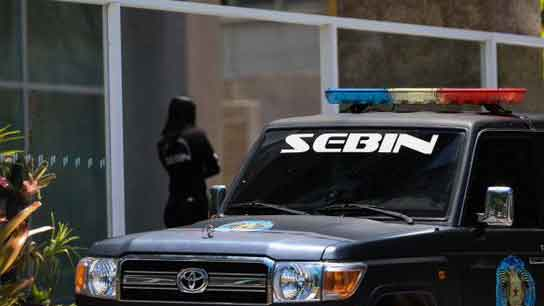
\includegraphics[width=300px]{229.jpg}%
\newline%
%
Caracas.{-}~Jeferson Esqueda, hermano del primer teniente de la aviación Carlos Esqueda, denunció a través de un video publicado en Twitter que su padre fue detenido por el Servicio Bolivariano de Inteligencia Nacional (Sebin) y desconocen su paradero.%
\newline%
%
Además, indicó que su familia está siendo perseguida y que su cuñada, quien tenía pocas semanas de embarazo,~ fue amenazada por los funcionarios con quitarle a los niños, acción que le produjo la pérdida de su bebé.%
\newline%
%
"El día sábado se llevaron a mi cuñada Mariel de Esqueda quien tenía pocas semanas de embarazo y la hicieron abortar amenazando con que se iban a llevar a los niños”, detalló.%
\newline%
%
También dijo que este domingo allanaron y destrozaron su casa, en Cagua, estado Aragua, desde donde se llevaron a su padre.~En sus declaraciones pidió a las organizaciones internacionales que intercedan.%
\newline%
%
“La destrozaron y se llevaron preso a mi papá Carlos Esqueda y no sabemos nada de dónde se encuentra (...) A las organizaciones internacionales, ayúdennos, por favor, auxilio",~clamó.%
\newline%
%
El paradero de su hermano~también se desconoce, después de su detención a pocas horas de ser liberado el pasado jueves.%
\newline%
%
Por su parte, Estela Lugo, hermana del primer teniente Luis Lugo, vía Twitter recordó que su hermano había sido capturado por la Dirección General de Contrainteligencia Militar (Dgcim) y que se encuentra con su padre y su cuñada, también detenidos, en Boleíta%
\newline%
%
“Mi hermano en  estos momentos se encuentra en Boleíta junto a mi padre y a su novia, hago responsable de la vida de mi familia a la Dgcim y a Nicolás Maduro”, expresó.%
\newline%
%
\end{document}